%\documentclass[iop,apj]{emulateapj}
\documentclass[preprint]{aastex}
\usepackage{times}
\usepackage{graphicx}
%\usepackage{fixltx2e}
\usepackage{astrobib_mnras2e}
\usepackage{lineno}

%% preprint2 produces a double-column, single-spaced document:

%% \documentclass[preprint2]{aastex}

%% Sometimes a paper's abstract is too long to fit on the
%% title page in preprint2 mode. When that is the case,
%% use the longabstract style option.

%% \documentclass[preprint2,longabstract]{aastex}

%% If you want to create your own macros, you can do so
%% using \newcommand. Your macros should appear before
%% the \begin{document} command.
%%
%% If you are submitting to a journal that translates manuscripts
%% into SGML, you need to follow certain guidelines when preparing
%% your macros. See the AASTeX v5.x Author Guide
%% for information.

\newcommand{\cpp}{c_{\perp}}
\newcommand{\cll}{c_{||}}
\newcommand{\dpp}{d_{\perp}}
\newcommand{\gmod}{g_{\rm mod}}
\newcommand{\rmod}{r_{\rm mod}}
\newcommand{\imod}{i_{\rm mod}}
\newcommand{\gcmod}{g_{\rm cmod}}
\newcommand{\rcmod}{r_{\rm cmod}}
\newcommand{\icmod}{i_{\rm cmod}}
\newcommand{\ipsf}{i_{\rm psf}}
\newcommand{\zpsf}{z_{\rm psf}}
\newcommand{\zmod}{z_{\rm mod}}
\newcommand{\rpsf}{r_{\rm psf}}
\newcommand{\ifib}{i_{\rm fib2}}

%% You can insert a short comment on the title page using the command below.

%\slugcomment{Not to appear in Nonlearned J., 45.}

%% If you wish, you may supply running head information, although
%% this information may be modified by the editorial offices.
%% The left head contains a list of authors,
%% usually a maximum of three (otherwise use et al.).  The right
%% head is a modified title of up to roughly 44 characters.
%% Running heads will not print in the manuscript style.

\shorttitle{Galaxy Target Selection in BOSS}
\shortauthors{Padmanabhan et al.}

%% This is the end of the preamble.  Indicate the beginning of the
%% paper itself with \begin{document}.

\begin{document}
\topmargin-1cm
\linenumbers

%% LaTeX will automatically break titles if they run longer than
%% one line. However, you may use \\ to force a line break if
%% you desire.

\title{Galaxy Target Selection for the SDSS-III Baryon Oscillation Spectroscopic
        Survey}

%% author and affiliation information.
%% Note that \email has replaced the old \authoremail command
%% from AASTeX v4.0. You can use \email to mark an email address
%% anywhere in the paper, not just in the front matter.
%% As in the title, use \\ to force line breaks.

\author{Nikhil Padmanabhan}
\affil{Dept. of Physics, Yale University, 260 Whitney Ave, New Haven, CT 06511}

%% Notice that each of these authors has alternate affiliations, which
%% are identified by the \altaffilmark after each name.  Specify alternate
%% affiliation information with \altaffiltext, with one command per each
%% affiliation.

%\altaffiltext{1}{Visiting Astronomer, Cerro Tololo Inter-American Observatory.
%CTIO is operated by AURA, Inc.\ under contract to the National Science
%Foundation.}

%% Mark off your abstract in the ``abstract'' environment. In the manuscript
%% style, abstract will output a Received/Accepted line after the
%% title and affiliation information. No date will appear since the author
%% does not have this information. The dates will be filled in by the
%% editorial office after submission.

\begin{abstract}
BOSS galaxies are great. 
\end{abstract}

%% Keywords should appear after the \end{abstract} command. The uncommented
%% example has been keyed in ApJ style. See the instructions to authors
%% for the journal to which you are submitting your paper to determine
%% what keyword punctuation is appropriate.

%\keywords{globular clusters: general --- globular clusters: individual(NGC 6397,
%NGC 6624, NGC 7078, Terzan 8}

\section{Introduction}

The Baryon Oscillation Spectroscopic Survey (hereafter BOSS, CITE???) is a
wide-field redshift survey designed to measure the expansion rate of the
Universe using the Baryon Acoustic Oscillation (BAO) method. On completion, BOSS
will have measured redshifts to 1.5 million galaxies and 160,000 quasars over
10,000 deg$^2$. This will allow a 1\% distance measurement using the BAO method
at z=0.35 and z=0.6 from the galaxy sample, as well as a 1.5\% distance
measurement at z=2.5 using the quasar sample. BOSS started taking spectroscopic 
data in September 2009, and is scheduled to complete in 2014. The first
spectroscopic data release from BOSS (DR9) is scheduled for July 2012; the first
cosmological results (CITES here????) were submitted in April 2012.
This paper sets out to document the algorithms used to select the BOSS galaxy
sample and describe its use as well as to describe the basic properties of the
galaxy sample.

There are three properties that determine the performance of a galaxy sample for
BAO measurements - the number density of the sample, the volume it covers, and
its large-scale clustering amplitude. These are usefully combined into the
effective volume of the sample (??? EFFECTIVE VOLUME EQN ????). Increasing the
effective volume of the sample directly increases the cosmological constraining
power of the sample. The requirements on the BOSS galaxy sample were to obtain
a sample of objects with a constant number density of $3 \times 10^{-4} h^{3}
\rm{Mpc}^{-3}$ out to z=0.6 (CHECK THIS EXACT CUT OFF????), falling off with a
magnitude limit at higher redshifts. 

Using the most luminous and most massive galaxies is an
efficient way to select samples optimized to be cosmological tracers. These
galaxies can be selected with low contamination rates from multiband imaging
data, and their redshifts may be obtained relatively efficiently. This is 
not a new observation; the Sloan Digital Sky Survey (SDSS) Luminous Red Galaxy
(LRG) sample (CITE???) and the 2SLAQ (2dF-SDSS LRG and Quasar, CITES???) used 
exactly such criteria to select samples of objects. BOSS extends these samples
in one important direction : while the SDSS LRG and 2SLAQ samples explicitly
targeted red galaxies, BOSS attempts to select a complete sample of massive
galaxies {\it irrespective} of their color. 

This paper is organized as follows FINISH THIS????

\section{The Sample Selection}

\subsection{Imaging Data}

The Sloan Digital Sky Survey (SDSS-I/II) imaged ??,000 deg$^2$ of the sky in 
the $ugriz$ bands using a specially designed camera on the 2.5m telescope at 
Apache Point Observatory in New Mexico. The SDSS-III project obtained additional
imaging for ?,000 deg$^2$ if sky in the Southern Galactic Hemisphere. As part
of this imaging effort, the original SDSS-I/II data and the SDSS-III data were
reduced with the latest versions of the SDSS image processing and calibration
pipelines. These data were released as part of Data Release 8 (CITE), and
a 10,000 deg$^2$ subsample of high Galactic latitude, low extinction data is 
the parent imaging catalog for the BOSS galaxy target selection. We note that
there are a number of differences between the reductions common to DR7 and DR8
(see the DR8 paper CITE for a detailed discussion); reproducing the BOSS galaxy
sample requires using the DR8 sample. 

The SDSS imaging pipeline returns a number of different estimates of the
photometry of galaxies. We briefly describe the ones used in the galaxy target
selection here; longer descriptions may be found on the SDSS website
\footnote{\texttt{http://www.sdss3.org/dr8}} and in relevant data release papers
(CITES HERE???). In all cases, all magnitudes have been corrected for Galactic
extinction (CITE SFD?????). 

The colors of galaxies are based on SDSS model magnitudes (denoted by the
subscript mod). These are determined by using the best-fit (psf-convolved)
deVaucouleurs or exponential profile fit in the $r$ band to determine the fluxes
in the other bands. Cuts in apparent magnitude are made with ``cmodel''
magnitudes (denoted by a subscript cmod). These are a linear combination of the
flux from the best fit exponential and deVaucouleur profile fit in each band
separately\footnote{contrasted with model magnitudes where the fit in the $r$
band is used} 
\begin{equation}
f_{\rm cmod} = (1 - P) f_{\rm exp} + P f_{\rm deV} \, , 
\end{equation}
where $P$ is the probability of an exponential or deVaucouleur profile
(reported as ${\rm frac}_{\rm deV}$ by the SDSS pipelines), and $f$ represents
the flux ({\it not magnitude}) assuming an exponential or deVaucouleur profile. 
Star-galaxy separation compares the PSF magnitudes of galaxies (denoted by a
subscript PSF) with model or cmodel magnitudes; PSF magnitudes underestimate the 
flux from extended sources compared with the model fits. Finally, we use 
``fiber2'' (denoted by subscript fib2) magnitudes to estimate the expected flux
through the SDSS-III 2'' fibers. 

The parent sample for the BOSS galaxy target selection is constructed by
selecting all detected objects that the photometric pipeline classifies as
galaxies, and that are ``resolved'' to be PRIMARY (i.e. either the only or the
best observation of this object; see the DR8 documentation for more details). We
do not make any cuts on photometricity at this stage; users constructing their
own samples for science analyses are advised to use the CALIB\_STATUS flag to
cut on photometricity (restricting to photometric observations corresponds to
\texttt{CALIB\_STATUS==1}). We also cull objects with suspect photometry as
reported in the flags set by the imaging pipeline. In particular, we require
\begin{enumerate}
  \item Objects that are flagged as detected in the $r$ and $i$ bands i.e. they
  have one of the BINNED1, BINNED2 or BINNED4 flags set in both the $r$ and $i$ bands.
  \item Objects not to be saturated :\texttt{(NOT SATUR) OR (SATUR AND (NOT
  SATUR\_CENTER))}
  \item Blended objects : \texttt{(NOT BLENDED) OR (NOT NODEBLEND)}
  \item Other photometric quality flags : \texttt{(NOT BRIGHT) AND (NOT
  TOO\_MANY\_PEAKS) AND (NOT PEAKCENTER) AND (NOT NOTCHECKED) AND (NOT
  NOPROFILE)}
\end{enumerate}

HIGHLIGHT CHANGE IN RESOLVE, AND HOW DO YOU FIX THIS. 


\subsection{Color Definitions}

In order to succintly describe the galaxy target selection, it is convenient to
define a set of auxiliary colors that track the locus of a passively evolving
population of galaxies in $gri$ color space. Following CITE Eisenstein et al???
and Cannon et al???? CITE, we define 
\begin{eqnarray}
\cll & = &  0.7 (\gmod - \rmod) + 1.2(\rmod - \imod - 0.18)  \\
\cpp & = & (\rmod - \imod) - (\gmod - \rmod)/4.0 - 0.18 
\end{eqnarray}
to describe the low redshift locus and 
\begin{eqnarray}
\dpp & = & (\rmod - \imod) - (\gmod - \rmod)/8 \,,
\end{eqnarray}
to describe the high redshift locus. As discussed above, the colors are defined
using SDSS model magnitudes, and are extinction-corrected. As was discussed in
Eis et al CITE??, the two sets of colors are necessary to describe the color
locus first when the 4000\AA\ break is in the SDSS $g$ band and then when it
redshifts into the $r$ band at $z\sim0.4$. This naturally divides target
selection into low and high redshift samples divided approximately at
$z\sim0.4$. 

Figure ???? plots these colors compared with both the stellar locus,
as well as a population of passively evolving galaxies. We see that $\cll$ runs
parallel to the low redshift galaxy locus, while $\cpp$ is approximately
perpendicular to it. The high redshift locus is described by $\dpp$ which runs
parallel to it. 

\begin{figure}
\caption{Figure showing the various colors compared to galaxy and stellar loci.}
\label{fig:color}
\end{figure}

\subsection{The LOWZ sample}

The low redshift (denoted LOWZ) sample is designed to be a straightforward
extension of the SDSS-I/II Cut I Luminous Red Galaxy Sample (CITE???).
WRITE DOWN PRINCIPAL CUTS AND MOTIVATION BEHIND THEM - ISOLATING THE GALAXY
LOCUS AND THEN A COLOR MAGNITUDE CUT TO GET AN SELECT THE BRIGHTEST OBJECTS. 
CUT TUNED TO GET AN APPROXIMATELY VOLUME LIMITED SAMPLE. ALSO DESCRIBE MAGNITUDE
LIMITS OF THE SAMPLE.

STAR GALAXY SEPARATION.

DESCRIBE OVERLAP WITH SDSS-I/II SAMPLE. HOW BIG IS THIS OVERLAP? WE DO NOT
TARGET GALAXIES ALREADY OBSERVED IN SDSS-I/II.

DESCRIBE TS BUG. GIVE SIMPLE PRESCRIPTION FOR SKIPPING IT. SEE APPENDIX FOR
DETAILS.

\subsection{The CMASS sample}

EXPLAIN BASIC MOTIVATION BEHIND THE CMASS SAMPLE -- EXTEND CUT II LRGS AND 2SLAQ
LRGS. REMOVE COLOR CUT

EXPLAIN DPERP CUT AND SLIDING COLOR MAGNITUDE CUT

\begin{figure}
\caption{Figure showing imag vs dperp and all the various cuts we make, marked.}
\end{figure}

EXPLAIN STAR GALAXY SEPARATION -- ORIGINAL AND ADDED Z-BAND CUT.

\begin{figure}
\caption{Figure motivating the z-band star galaxy separation}
\end{figure}

EXPLAIN IFIBER2 CUT.

\subsection{Sparse Sampling Cuts}

LIST THE CUTS HERE AND MOTIVATION

\subsection{Summary of Target Selection}

We summarize the two target selection algorithms here. The LOWZ targets are
defined by 
\begin{eqnarray}
\rcmod  & < & 13.5 + \cll/0.3 \\ 
|\cpp| & < & 0.2 \\
16 & < \rcmod < & 19.6 \\
\rpsf - \rcmod & > & 0.3 \,\,,
\end{eqnarray}
while the CMASS objects are selected by 
\begin{eqnarray}
\icmod & < & 19.86 + 1.6(\dpp - 0.8) \\
17.5 & < \icmod <  & 19.9 \\
\dpp & > & 0.55 \\
\ipsf - \imod & > & 0.2 + 0.2(20 - \imod) \\
\zpsf - \zmod & > & 9.125 - 0.46 \zmod \\
\rmod - \imod & < & 2 \\
\ifib & < & 21.5 \,\,.
\end{eqnarray}
The SPARSE sample extends the CMASS sample selection by altering the sliding
$\icmod$-$\dpp$ cut to 
\begin{eqnarray}
\icmod & >= & 19.86 + 1.6(\dpp - 0.8) \\
\icmod & < & 20.14 + 1.6(\dpp - 0.8) \,\,, 
\end{eqnarray}
with the other cuts unchanged. These galaxies are further subsampled down to a
number density of 5/deg$^2$. 

\subsection{Sample Usage}

EXPLAIN BOSSTARGET1 AND ALL THE BITS

TRACK DOWN WHEN ONE OF THE BOSSTARGET1 BITS GOT OVERLOADED.

\section{Sample Properties}

\begin{figure}
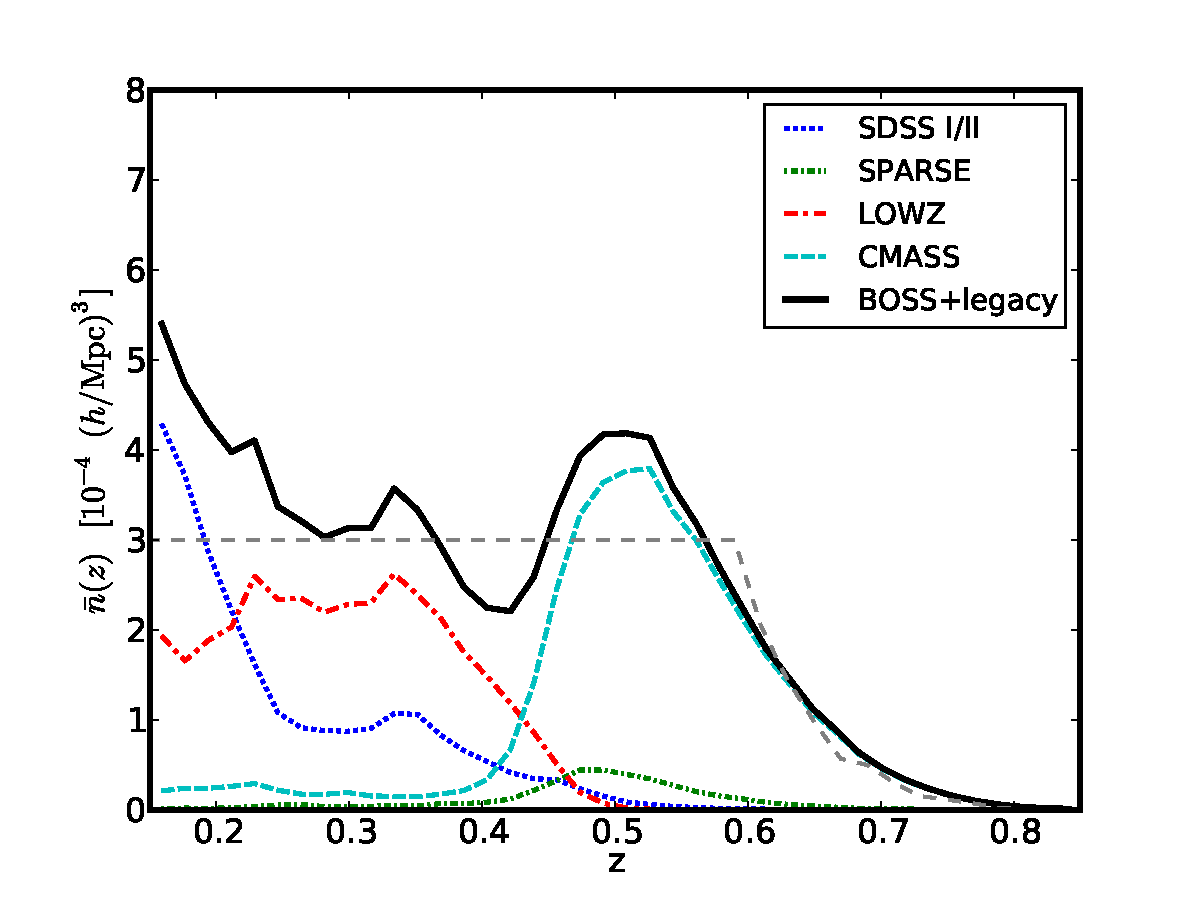
\includegraphics[width=0.95\columnwidth]{plots/nbarz-40-chunk6-21-CMASS_LOWZ_SPARSE}
\caption{The number densities of the Legacy, LOWZ and CMASS, and SPARSE 
galaxies. The LOWZ curve plotted here only includes {\it new} galaxies targeted
by BOSS, and does not include the Legacy targets. These are a
significant fraction of all the LOWZ targets. The BOSS+Legacy curve represents
the full BOSS sample, including both galaxies with spectra obtained by BOSS and
those with existing spectra. We observe that the BOSS galaxy target selection is
meeting its target goal (thin dashed lines).}
\label{fig:nbar}
\end{figure}

\begin{figure}
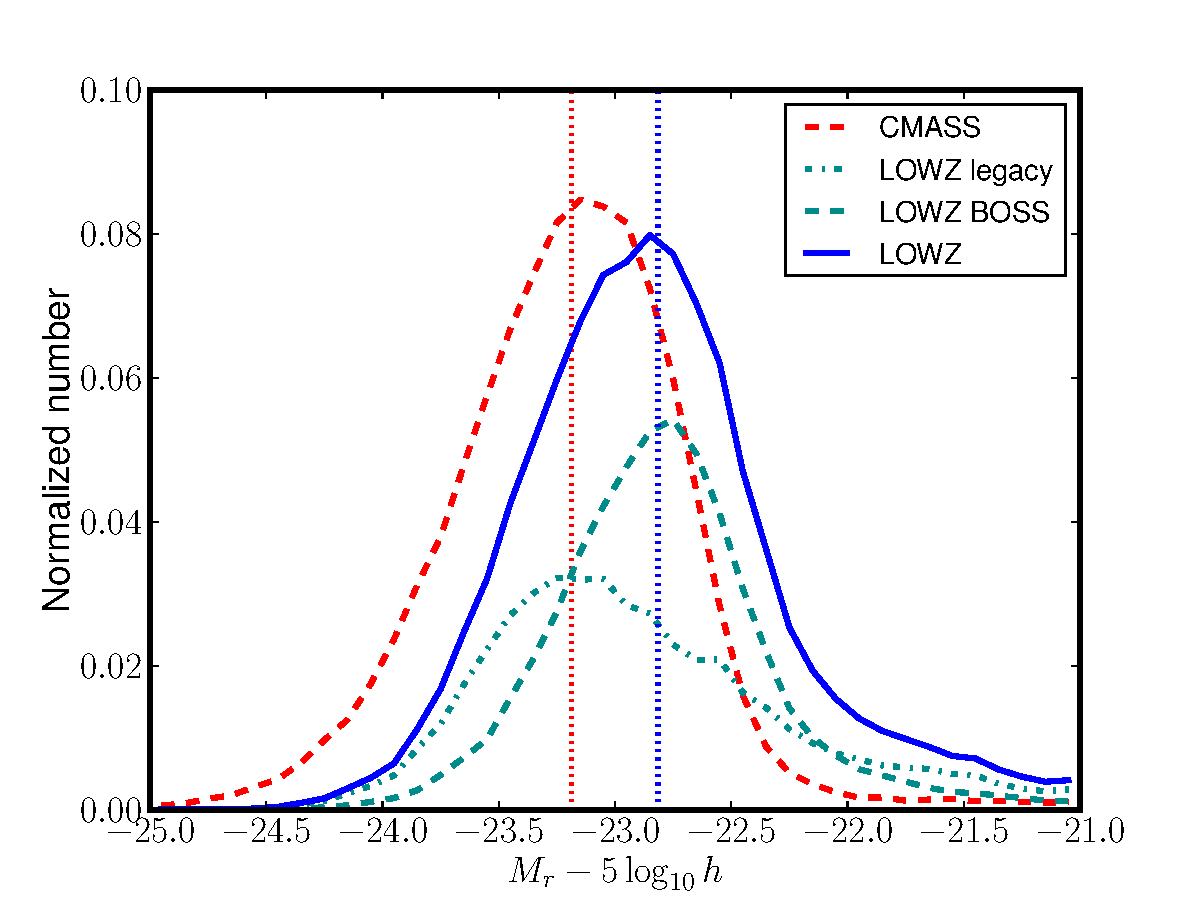
\includegraphics[width=0.95\columnwidth]{plots/LOWZ-r_absmag}
\caption{The absolute rest-frame $r$ band magnitudes of LOWZ and CMASS
galaxies. These magnitudes are k-corrected using the NEED DETAILS FROM JOHN
HERE????. The vertical lines plot the median magnitudes of both samples.We
subdivide the LOWZ sample into the Legacy SDSS-I/II galaxies and galaxies with spectra 
obtained by BOSS. As designed, the newer galaxies are
$\sim$ 0.5 magnitudes fainter.}
\label{fig:absmag}
\end{figure}

\begin{figure}
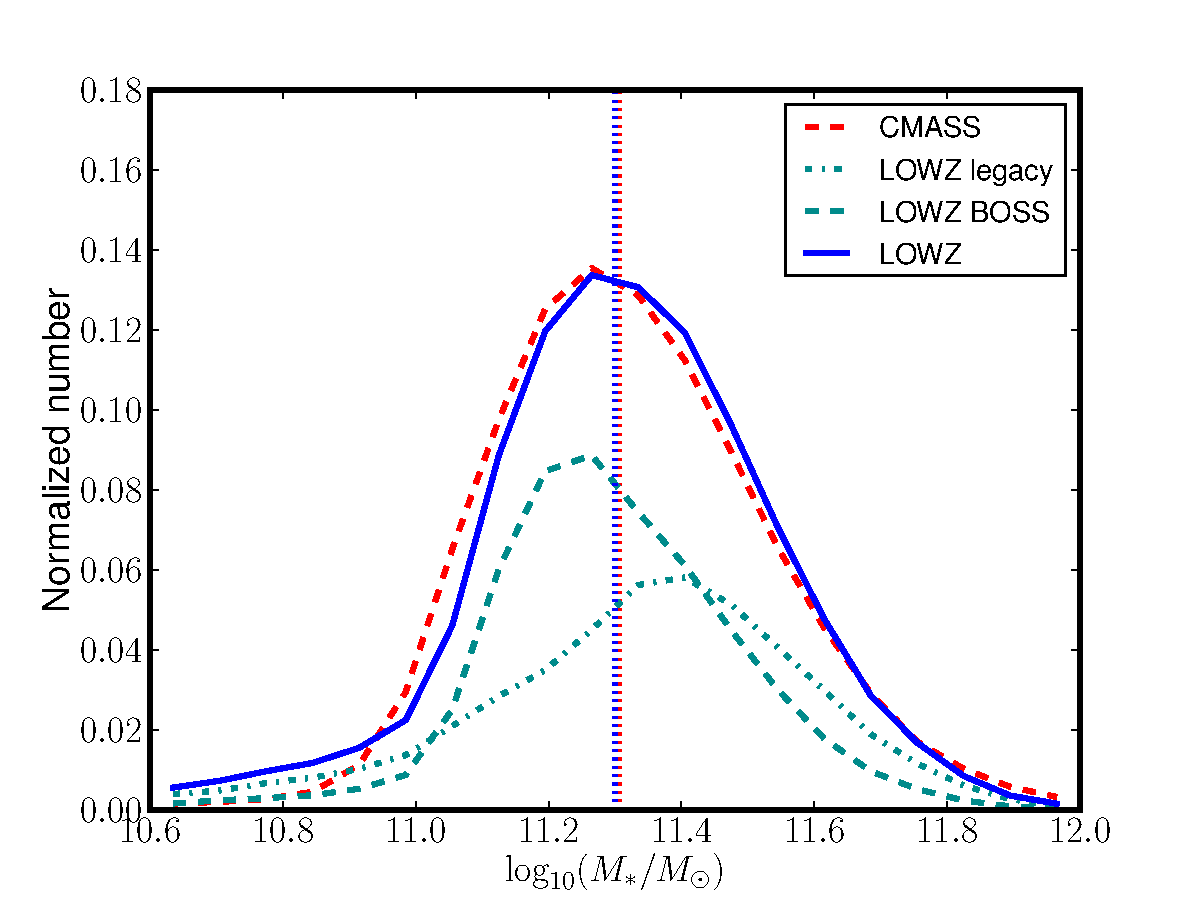
\includegraphics[width=0.95\columnwidth]{plots/LOWZ-stellarmass}
\caption{The stellar masses of the LOWZ and CMASS galaxies, obtained using NEED
DETAILS HERE????. The vertical lines show the median ???? stellar mass of both
samples. We find that both samples have very similar stellar mass distributions.
As in Fig.~\ref{fig:absmag}, we separate the LOWZ sample into Legacy and BOSS
galaxies and find that the BOSS galaxies }
\label{fig:stellarmass}
\end{figure}

DISCUSS NUMBER DENSITIES AND ABSOLUTE MAGNITUDES

DISCUSS NORTH V SOUTH (OR JUST REFERENCE PAPERS ON THIS).

\section{Conclusions}


\section{Acknowledgments}

Funding for SDSS-III has been provided by the Alfred P. Sloan
Foundation, the Participating Institutions, the National Science
Foundation, and the U.S. Department of Energy Office of Science. The
SDSS-III web site is http://www.sdss3.org/.

SDSS-III is managed by the Astrophysical Research Consortium for the
Participating Institutions of the SDSS-III Collaboration including the
University of Arizona,
the Brazilian Participation Group,
Brookhaven National Laboratory,
University of Cambridge,
Carnegie Mellon University,
University of Florida,
the French Participation Group,
the German Participation Group,
Harvard University,
the Instituto de Astrofisica de Canarias,
the Michigan State/Notre Dame/JINA Participation Group,
Johns Hopkins University,
Lawrence Berkeley National Laboratory,
Max Planck Institute for Astrophysics,
Max Planck Institute for Extraterrestrial Physics,
New Mexico State University,
New York University,
Ohio State University,
Pennsylvania State University,
University of Portsmouth,
Princeton University,
the Spanish Participation Group,
University of Tokyo,
University of Utah,
Vanderbilt University,
University of Virginia,
University of Washington,
and Yale University.

\appendix

\section{Commissioning Data}
\label{app:comm}

EXPLAIN THE ORIGINAL COMMISSIONING CUTS (ONLY FOR DATA WE PLAN ON RELEASING). 


\section{Changes in Galaxy ``RESOLVE''}
\label{app:resolve}

DESCRIBE THE CHANGES HERE. DOCUMENT WHEN THE CHANGE HAPPENED, AND HOW THIS 
GETS SOLVED IN THE DATA RELEASE.

\begin{figure}
\caption{An Aitoff projection showing the regions of sky where the primary
objects changed. MAKE THIS FIGURE.}
\end{figure}

\section{A Bug in the LOWZ Galaxy Selection}
\label{app:lowzbug}

DESCRIBE THE BUG IN DETAIL. WHAT CUT WAS EXACTLY MADE? WHAT DATA DID IT EFFECT?
SHOW THE EFFECT ON THE NUMBER DENSITY OF TARGETS. REPEAT HOW ONE CAN AVOID THIS.


\end{document}

